\documentclass[12pt]{article}
\usepackage[utf8]{inputenc}
\usepackage[T1]{fontenc}
\usepackage[francais]{babel}
\usepackage{graphicx}

\title{\textbf{Projet Réseaux : Chatroom\\PYTHON3 TCP/IP SELECT\\ (2018-2019)}}
\author{\textbf{GEOFFROY Kirsan, HOAREAU Martin}}

\begin{document}
\maketitle

\tableofcontents

\begin{abstract}
    Le but de ce mini-projet est d'implémenter un serveur client chat d'abord minimale, puis ensuite amélioré. 
    On a repris le serveur de chat vu en cours que l'on a étendu. L'idée était de se rapprocher du protocole IRC(RFC1459). 
    Le serveur gère différentes conversations dans des canaux dédiés ("Channel" en IRC). Un client ne peut communiquer que dans un seul canal à la fois.\\ 
    À travers ce rendu, nous allons vous expliquer comment nous sommes parvenu à nos fins grâce à nos méthodes d'approche, les difficultés rencontrées et leurs solutions.
\end{abstract}

\section{Réfléxion}
Pour commencer, nous utilisons le protocole TCP/IP, ce situant dans la couche 4 du modèle OSI de référence. Il permet une communication rapide, convient pour un transfert d'un nombre moyen de données (parfaites pour un chat), peut-être utilisés vers un système d'autres marque et il offre un moyen d'acquittement. \\
Ensuite, nous avons dû réfléchir à comment utiliser les outils à notre disposition, c'est-à-dire comment stocker les différentes données qui nous seront utiles.Pour débuter, nous voulions faire un dictionnaire de dictionnaire avec en clé le socket et en valeur un dictionnaire prenant des clés telles que addr ,nick, channel, admin et associant à chacun la valeur correspondante.
Cela nous a vite causé beaucoup de problèmes de compréhension dans notre façon d'accéder aux éléments souhaités. Nous avons donc décidé d'abandonner cette façon et nous sommes rendu compte qu'il y a plus simple. 
Notamment en passant une liste en tant que valeur d'un dictionnaire.Au final, nous utilisons donc deux dictionnaires un qui va nous permettre de gérer les clients, l'autre les channels.\\
Respectivement leur (clé:valeur) est : (Socket:[addr,"nick","channel","admin"]) et (Channel:[]) avec :
\begin{enumerate}
    \item dico-client value : addr = Addresse, nick = nickname du client, channel  = channel actuel du client, admin = booléen -> True si admin, False sinon.
    \item dico-channel key : Nom du channel ; value : [] = liste vide, chaque fois qu'un client rejoint un channel, on ajoute la socket à cette liste.
\end{enumerate}
Ainsi, nous pouvons passer du dico-channel au dico-client et vice-versa grâce au socket.\\De plus, nous avons une liste stockant toutes les sockets connectés au serveur et une liste stockant tous les nicks-names présent sur le serveur.De cette façon, nous pouvons facilement permettre des nicks uniques et fermer les connexions.\\
Nous avons décidé de gérer toutes les commandes côtés serveur afin de laisser un client simple et minimaliste qui tape juste des messages, si ce message et une commande alors le serveur l'interprétera sinon il enverra le message à tous les clients.

\section{Client}
Dans cette section nous allons nous intéresser à la partie client du réseau. Notre client est ce qu'il y a de plus minimaliste. Nous avions commencé à coder des commandes côté serveur et coter client.Ceci n'était pas clair pour nous donc nous avons décidé d'implémenter toutes les commandes côté serveur pour une question de clarté de notre fichier client.\\
Tout d'abord dans notre fichier client nous lui demandons d'indiquer un nom d'utilisateur, nous essayons la connexion au serveur si celle-ci et effectué nous envoyons notre nom d'utilisateur au serveur qui va le réceptionner et le stocker dans ses dictionnaires et liste respectives.
Ensuite nous gérons simplement 2 cas; si un message arrive du serveur nous allons l'afficher côté client ou si l'utilisateur entre un message comme une commande ou un message quelconque nous allons l'envoyé à notre serveur. Ceci dit notre client à quelques petits problèmes, nous n'arrivons pas à faire en sorte que lorsque le client effectue "ctrl+c" sa connexion s'arrête brutalement.
Pour le serveur c'est comme si le client n'avait rien écrit. Ceci doit venir de notre fichier client py mais nous n'arrivons pas à résoudre entièrement ce problème.Lorsque nous le résolvons d'autres problèmes apparaissent tels que le serveur ne peut pas recevoir de multiples clients. Nous avons donc laissé ce problème non majeur de coté pour se préoccuper des problèmes plus importants. 

\section{Serveur}
\subsection{Commandes V0}
Ici nous allons voir les différentes commandes et les problèmes qu'elles ont causés (ou non).\\
\begin{itemize}
    \item KICK <nick> - Pour la réalisation de cette commande un temps de réflexion était nécessaire. Tout d'abord nous traitons les différents cas d'erreur ("Nick not indicated", "You don't have the permisssion [admin]","Invalid nickname","You can't kick a user 
    which is not currently in a channel"). Ensuite nous parcourons les sockets présentes dans le channel courant afin d'identifier la socket correspondant au <nick> indiqué en paramètre. Une fois celle-ci identifiée nous allons la supprimer du channel
    courant pour l'ajouter au channel "Default". Nous lui retirons ses droits d'administrateur s'il en avait, puis nous lui envoyons un message disant qu'il s'est fait exclure du channel.\\
    \item JOIN <channel> - Cette commande permet de rejoindre un channel. S'il existe, ont le rejoint sinon on le créer et le client l'ayant créé se voit devenir administrateur de ce channel.\\
    Le problème rencontré lors de cette fonction était subtil. En effet dans la V0 il n'est pas possible d'être connecté à plusieurs channels, un client est associé à un channel. Donc si on fait un JOIN sur un channel
    puis un JOIN sur un autre, on sort du premier pour rejoindre le deuxième. Ainsi, il était possible de laisser des channels fantome : c'est-à-dire vide. Pour régler cela, nous avons décidé de dire que pour JOIN un channel,
    il ne faut pas déjà être dans un channel : si on essaye, alors un message indiquant quoi faire apparaît. \\
    \item WHO - Aucun problème rencontré lors de l'implémentation de cette fonction. Nous utilisons une boucle for pour parcourir la liste des sockets présentes dans le channel courant, puis nous envoyons à l'utilisateur la liste des nick "sock.send((dico client[i][1]))" 
    présent dans le channel courant.\\
    \item BYE - Quelques problème rencontrés lors de la réalisation de cette commande. Lorsque nous faisions un sock.sendall(...) le client se fermer brutalement comme s'il avait 
    "crash". Nous avons donc décidé d'enlever cette ligne de code ne sachant pas d'où venait le problème et de la remplacer par un simple print(...) du côté du serveur. Ensuite nous le supprimons de ces dictionnaires et listes respectives puis nous fermons sa socket.\\
    \item HELP - Aucun problème rencontré pour cette commande. À l'aide de sock.send(...) nous envoyons à l'utilisateur la liste des commandes disponible. \\
    \item LEAVE - La réalisation de cette commande est plus complexe que ce qu'on pensait. Plusieurs cas doivent être impérativement traités pour assurer un bon fonctionnement de la commande. L'utilisateur quitte le channel. Si le channel est vide, il est alors supprimé. 
    Cependant, si l'utilisateur est admin il faut laisser le droit d'admin à la personne ayant rejoint le channel après l'admin.
    Laisser le droit d'administrateur s'est révélé compliqué de réflexion mais tient en une ligne. En effet, nous avons eu du mal à visualiser comment accéder à ce champ, une feuille un stylo et une bonne heure nous ont permis d'en venir à bout. IMAGEANNEXE \\
    \item MSG <nick>  - Envoie un message privé à un utilisateur du channel ou se situe le client qui tape la commande. Comme nous avons "split" le message de l'utilisateur en un tableau de mot il nous a fallu un petit peu de réflexion pour réussir cette commande.
    Tout d'abord nous vérifions si la taille du message envoyé par l'utilisateur contient bien un <nick> passé en argument et un message à lui transmettre. Si c'est le cas alors on fait une boucle parcourant les sockets présentes dans le même channel que 
    l'utilisateur. Si on trouve un <nick> dans le channel courant alors on lui envoie le message privé que l'utilisateur souhaite lui transmettre. Pour ce faire nous regardons la taille du message, nous faisons une boucle parcourant cette taille puis nous 
    envoyons "sock.send(data[i])" qui est censé envoyer le message mot à mot.\\
    \item REN - Elle permet de renommer un channel. Or, une clé d'un dictionnaire est immuable, c'est-à-dire qu'on ne peux pas la modifier.\\ Pour surmonter cette contrainte,
    nous créons une nouvelle clé dans le dico-channel portant le nouveau nom désiré du channel, en valeur on lui passe les valeurs de l'ancien channel. Ensuite on supprime l'ancien channel et on fait une boucle for parcourant
    tous les clients qui étaient dans l'ancien channel et on modifie leurs champs channel avec le nom du nouveau.\\
    \item LIST - Pas de gros problème rencontré lors de la réalisation de cette commande. Il nous suffit simplement de parcourir la liste des channels existant "list(dico channel)" puis de les afficher un par un à l'utilisateur
    à l'aide de sock.send(...).\\
\end{itemize}

\subsection{Commandes V1}
Ici nous allons voir les différentes commandes mises en place ainsi que les problèmes rencontrés lors de la phase de codage de la V1.\\
Tout d'abord, nous avons commencé par une courte phase de réflexion pour faire une V1. Pour cette V1 nous avons modifié notre "dico client" pour lui ajouter une clé qui va servir à stocker la liste des channels auxquels notre client appartient ainsi que sa liste de booléen correspondant à ses droits [admin] en fonction du channel.\\
Exemple :  dico client[sock][4] = (["Default","Chan1","Chan2"],[False,True,False]) 
Car oui dans cette V1 un client peut se connecter à différent channels simultanément. Pour ajouter cette fonctionnalité au chatroom, nous avons donc modifié les commandes (JOIN, KICK, LEAVE, WHO, GRANT et l'envoie de message aux autres utilisateurs dans le channel courant) (reprisent de la V0) pour que ça fonctionne en toutes circonstances.\\
Les modifications à apporter ne sont pas énormes mais demandent tout de même un temps de réflexion pour ne pas faire n'importe quoi.\\

\begin{itemize}

    \item CURRENT : Pour cette commande, pas de gros problèmes particuliers rencontrés. Tout d'abord nous vérifions si l'utilisateur à entrer un argument à la commande , si ce n'est pas 
    le cas alors on lui "print" son channel courant. Sinon on vérifie si le <channel> passé en paramètre appartient à notre "dico client [sock][4][0]" liste de channel auquel le client appartient
    ou si le <channel> est déjà notre channel courant. Si ce n'est pas le cas alors on modifie la valeur de notre dico client contenant son channel courant par <channel> indiqué en paramètre.\\
    \item GRANT/REVOKE : Pour ces commandes, nous n'avons rencontré aucun problème particulier. Nous avons regroupé ces deux commandes car elles étaient à quelques lignes de code près , identiques. 
    Tout d'abord nous commençons à vérifier si l'utilisateur a bien indiqué un paramètre en argument de la commande (ex: /GRANT lulu). Si ce n'est pas le cas on lui envoie un message d'erreur.
    Sinon on vérifie si l'utilisateur a les droits pour effectuer cette commande [admin]. Si ce n'est pas le cas on lui renvoie un message d'erreur, sinon on parcourt la liste contenants 
    tout les nicknames présents sur le serveur et on regarde si le <nick> passé en paramètre appartient à cette liste. Si ce n'est pas le cas on renvoie un message d'erreur à l'utilisateur sinon
    on parcourt les sockets des personnes présentes dans le channel courant (qu'elles l'aient en courant ou juste dans leur liste), lorsqu'on trouve la socket du <nick> passé en paramètre on lui administre les droits d'administrateur où on lui retire
    les droits d'administrateur, ça dépend de la commande tapée (/GRANT où /REVOKE).\\
    \item NICK : Pour cette commande, nous commençons par vérifier que l'utilisateur ait bien indiqué un nouveau <nick> en argument. Ensuite on vérifie si le <nick> est identique à l'utilisateur ou 
    s'il est déjà présent dans notre liste de nick. Si ce n'est pas le cas alors on commence par supprimer son ancien <nick> de la "liste de nick", ensuite on modifie la valeur qu'occupe le <nick>
    dans notre "dico client" et on lui met le nouveau <nick> entré en paramètre de la commande. On àjoute ce nouveau <nick> à notre "list nick" puis on envoie un message de succès à l'utilisateur.\\

\end{itemize}

\subsection{Modifications apportées par rapport à la V0}
Comme dit précédemment nous avons dû modifier quelques commandes de la V0 pour pouvoir les adapter à notre nouvelle version de chatroom (Un client peut appartenir à de multiples canaux simultanément)\\

\begin{itemize}
    \item JOIN (Annexes 1):  On ne supprime pas la socket du channel courant lorsqu'on rejoins un nouveau channel existant ou non. 
    Le channel courant deviens celui que l'on viens de rejoindre. Ajoute le channel à la liste channel du client, si il le crée ajoute le booleen True à liste booleens du client,
    sinon ajoute le booléen False à la liste bool du client.\\
    \item LEAVE (Annexe 2): Tout d'abord nous regardons si la longueur de la liste channel du client est supérieur à 2 ou égale à 2.\\
     - Si elle est supérieur à deux alors, on récupère l'index du channel dans la liste channel du client . 
    Ensuite on supprime le channel quitté de la liste channel du client, et on supprime le booleen correspondant à l'index du client dans la list bool du client.
    Puis  On fixe le courant du client au premier channel rejoint après le channel qu'on quitte actuellement. \\
     - Si  elle est égale à deux alors, on supprime le channel de la list channel du client et supprime le booléen correspondant au channel quitté.
     Ensuite, on initialise le channel courant du client à "Default" ainsi que ses droits d'administrateur à "False".\\ 
    \item KICK : Les modifications apportés pour cette commande sont très similaires à celle apportés pour la commande "LEAVE". Nous avons simplement copier-coller 
    la partie de code de la commande LEAVE (voir annexe 3) dans la commande "KICK" en remplaçant "sock" par la socket du client que nous voulons éjecter du channel.\\
    \item WHO : Dans notre boucle on distingue désormais deux cas : le premier étant celui de la V0 (ça veut dire que les clients n'ont qu'un channel qui est leur channel courant) et le deuxième celui de la V1
    ou un client peut avoir plusieurs canaux. Donc on teste deux choses : on parcourt toutes les sockets de notre dico channel du channel de celui qui tape la commande : si le channel courant de celui qui tape la commande est le même que la socket
    qu'on regarde alors on l'affiche. Si ce n'est pas son channel courant alors on regarde si le channel de celui qui tape la commande est dans la liste de channel de la socket parcouru, si oui on l'affiche.
    \item MSG : Nous avons simplement ajouté une condition qui est d'envoyé un message à ceux donc le channel courant est identique à celui de l'expéditeur du message.\\
\end{itemize}

\section{Annexes}

\begin{figure}
\begin{center}
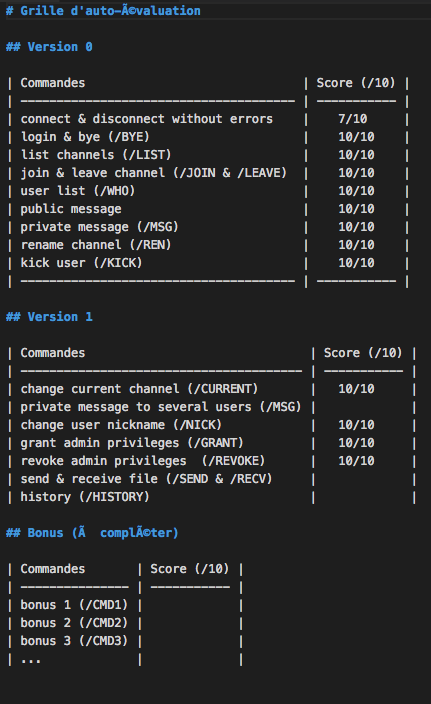
\includegraphics[height=10cm,width=7cm]{grille.png} 
\end{center}
\caption{Grille auto-évaluation}
\label{Grille auto-évaluation}
\end{figure}

\begin{figure}
\begin{center}
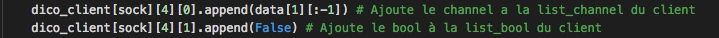
\includegraphics[width=15cm]{annexe1.png} 
\end{center}
\caption{Annexe 1}
\label{Annexe 1}
\end{figure}

\begin{figure}
\begin{center}
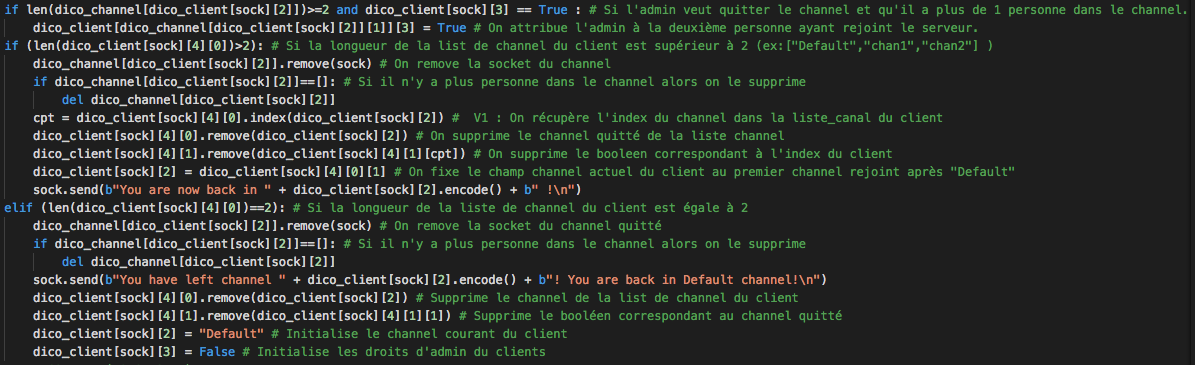
\includegraphics[width=15cm]{annexe2.png} 
\end{center}
\caption{Annexe 2}
\label{Annexe 2}
\end{figure}
            

\end{document}

